\section{Концепция построения подсистемы аутентификации пользователей в сети
корпоративных порталов с применением портативного цифрового ключа доступа}
\label{sect:concept}
В качестве базового алгоритма шифрования для процесса аутентификации был взят
алгоритм электронно-цифровой подписи (ЭЦП).

Рассмотрим то, от каких действий злоумышленника должна защищать система
шифрования на основе ЭЦП:
\begin{itemize}
  \item Отказ от выполненных действий. Субъект утверждает, что он не посылал
  некоторое сообщение, хотя на самом деле он его послал;
\item Модификация сообщения. Получатель
модифицирует полученное сообщение и утверждает, что именно такую версию
он и получил;
\item Подделка. Субъект фабрикует сообщение и утверждает, что оно ему
прислано;
\item Перехват. Злоумышленник С перехватывает сообщение, посланное А к В с
целью модификации;
\item Маскировка. Посылка сообщения от чужого имени;
\item Повтор.
Злоумышленник С посылает повторно сообщение от А к Б, перехваченное им ранее.
\end{itemize}

Решение практически всех этих проблем может быть реализовано с помощью
электронной подписи, базирующейся на алгоритме RSA.~\cite{ECP}

Пусть \textit{А} передает сообщение \textit{DATA} адресату \textit{Б}.
Электронная подпись отправителя \textit{А} базируется на его секретном ключе и
открытом ключе, которым обладает получатель \textit{Б}. Сначала отправитель с
помощью хэш-функции генерирует дайджест своего сообщения для приведения текста сообщения к фиксированной длине. Затем с помощью
своего секретного ключа он формирует электронную подпись. При этом \textit{А} не
может отказаться от того, что именно он послал сообщение, так как только он знает свой
секретный ключ. Электронную подпись нельзя использовать повторно и подписанный
документ нельзя модифицировать, так как любые модификации неизбежно изменят его
дайджест, а, следовательно, и электронную подпись. Получатель с помощью
открытого ключа дешифрует код электронной подписи, а затем с использованием
дайджеста проверяет ее корректность. Общая схема работы электронно-цифровой
подписи в контексте информационной системы представлена на рисунке
~\ref{ris:3.1.1}.

\begin{figure}[h]
\center{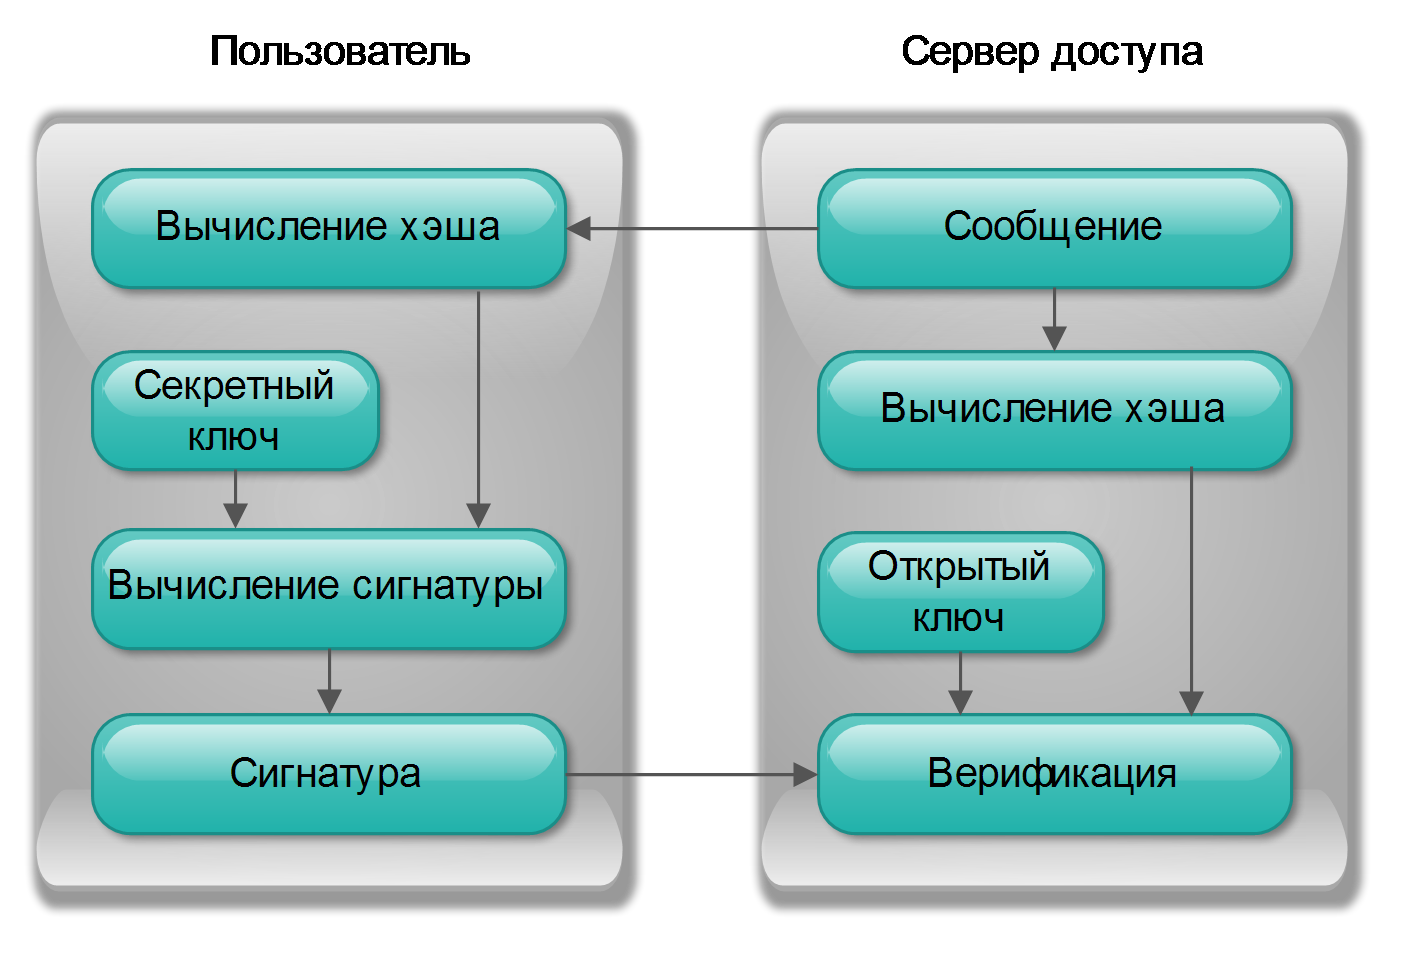
\includegraphics[width=1\linewidth]{3-1-1}}
\caption{Общая схема создания и верификации ЭЦП}
\label{ris:3.1.1}
\end{figure}

Процесс аутентификации на основе асимметричного алгоритма шифрования включает в
себя 3 макро-этапа:
\begin{itemize}
  \item Генерация ключей;
  \item Создание шифра к сообщению (документу);
  \item Верификация (проверка подлинности) самого сообщения и шифра.
\end{itemize}

Процесс генерации сопровождается заключением договора между удостоверяющим
центром и владельцем электронного ключа. Данный договор называется сертификатом и устанавливает
соответствие между открытым ключом и данными человека, однозначно
характеризующие его, и обладающего соответствующим ему (открытому ключу)
закрытым ключом. Потоки информационного обмена на данном этапе отражены на
рисунке~\ref{ris:3.1.2}.

\begin{figure}[h]
\center{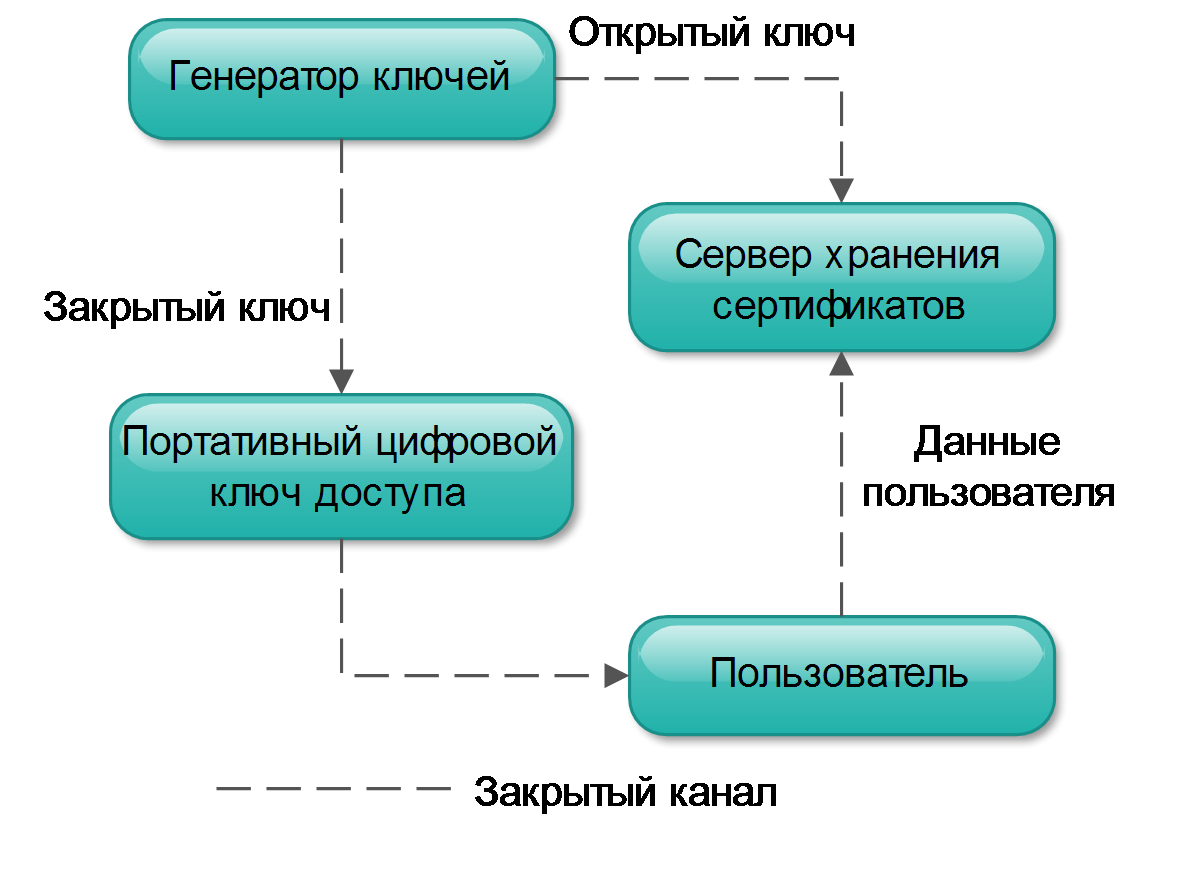
\includegraphics[width=1\linewidth]{3-1-2}}
\caption{Схема генерации индивидуального ключа}
\label{ris:3.1.2}
\end{figure}
  
Закрытый ключ является собственностью пользователя системы, их личным правом на
использование, имеющее юридическую силу, и не должен быть доступен другим людям
ни при каких обстоятельствах.  Поэтому цифровой носитель и алгоритм, осуществляющий генерацию
шифра, должен обеспечивать абсолютную секретность ключа и простейшие средства
безопасности, такие как:
\begin{itemize}
  \item полное скрытие ключа от визуального доступа на экране монитора при его
использовании;
  \item защита от нежелательной утраты цифрового носителя ключа,
вследствие чего он может стать доступен третьим лицам;
  \item защита от вредоносных
или шпионских программ, действующих неумышленно или целенаправленно на
компьютере, с которым работает пользователь в данный момент, для получения права
подписи от имени законного владельца закрытого ключа.
\end{itemize}

Для обеспечения поставленных требований необходимо разработать специальное
аппаратное устройство, которое возьмет на себя часть функций по организации
процессов информационного обмена и обеспечит защиту ключа на необходимом уровне,
которую невозможно достичь средствами наиболее распространённых операционных систем.
Кроме того, отдельное устройство должно быть сильно независимо от ПК, имееть
свою собственную память, к которой невозможно получить физический доступ и
обладать ограниченным набором команд.~\cite{evstifiev}
 
Данное устройство должно обладать следующими особенностями:
\begin{itemize}
  \item компактность, переносимость и малая себестоимость
изготовления;
\item устройство должно соединяться с ПК по средствам стандартных и наиболее
распространённых коммуникационных интерфейсов, используя стандартные протоколы
передачи данных. Речь идёт об использовании последовательного интерфейса USB. 
Недопустимо использовать интерфейсы, требующие дополнительного оборудования для
считывания данных с носителя ключа и не входящие в комплект стандартных
коммуникационных интерфейсов ПК, так как это снижает эффективность использования
данной технологии;
\item данное устройство должно иметь вычислительный механизм,
обладающий возможностью за относительно короткое время сгенерировать цифровую
подпись на основе закрытого ключа, <<спрятанного>> в памяти данного
устройства;
\item устройство-носитель закрытого ключа должно предоставлять единственный
интерфейс для установления связи только для определённого формата входных и
выходных данных, таким образом быть защищено от любого считывания данных из
памяти. На вход устройства подаётся сообщение в битовом виде. На выходе
получается сигнатура, которая имеет право быть
открытой и находиться в свободном обращении.
\end{itemize}  

Процесс вычисления сигнатуры (шифра) довольно сложный и выполняется в несколько
этапов, каждый из которых сопровождается информационным обменом различного рода.
Основной обмен информацией происходит между клиентской программой
(browser) и сервером доступа. Схема взаимодействий представлена на рисунке
~\ref{ris:3.1.3}.

\begin{figure}[h!]
\center{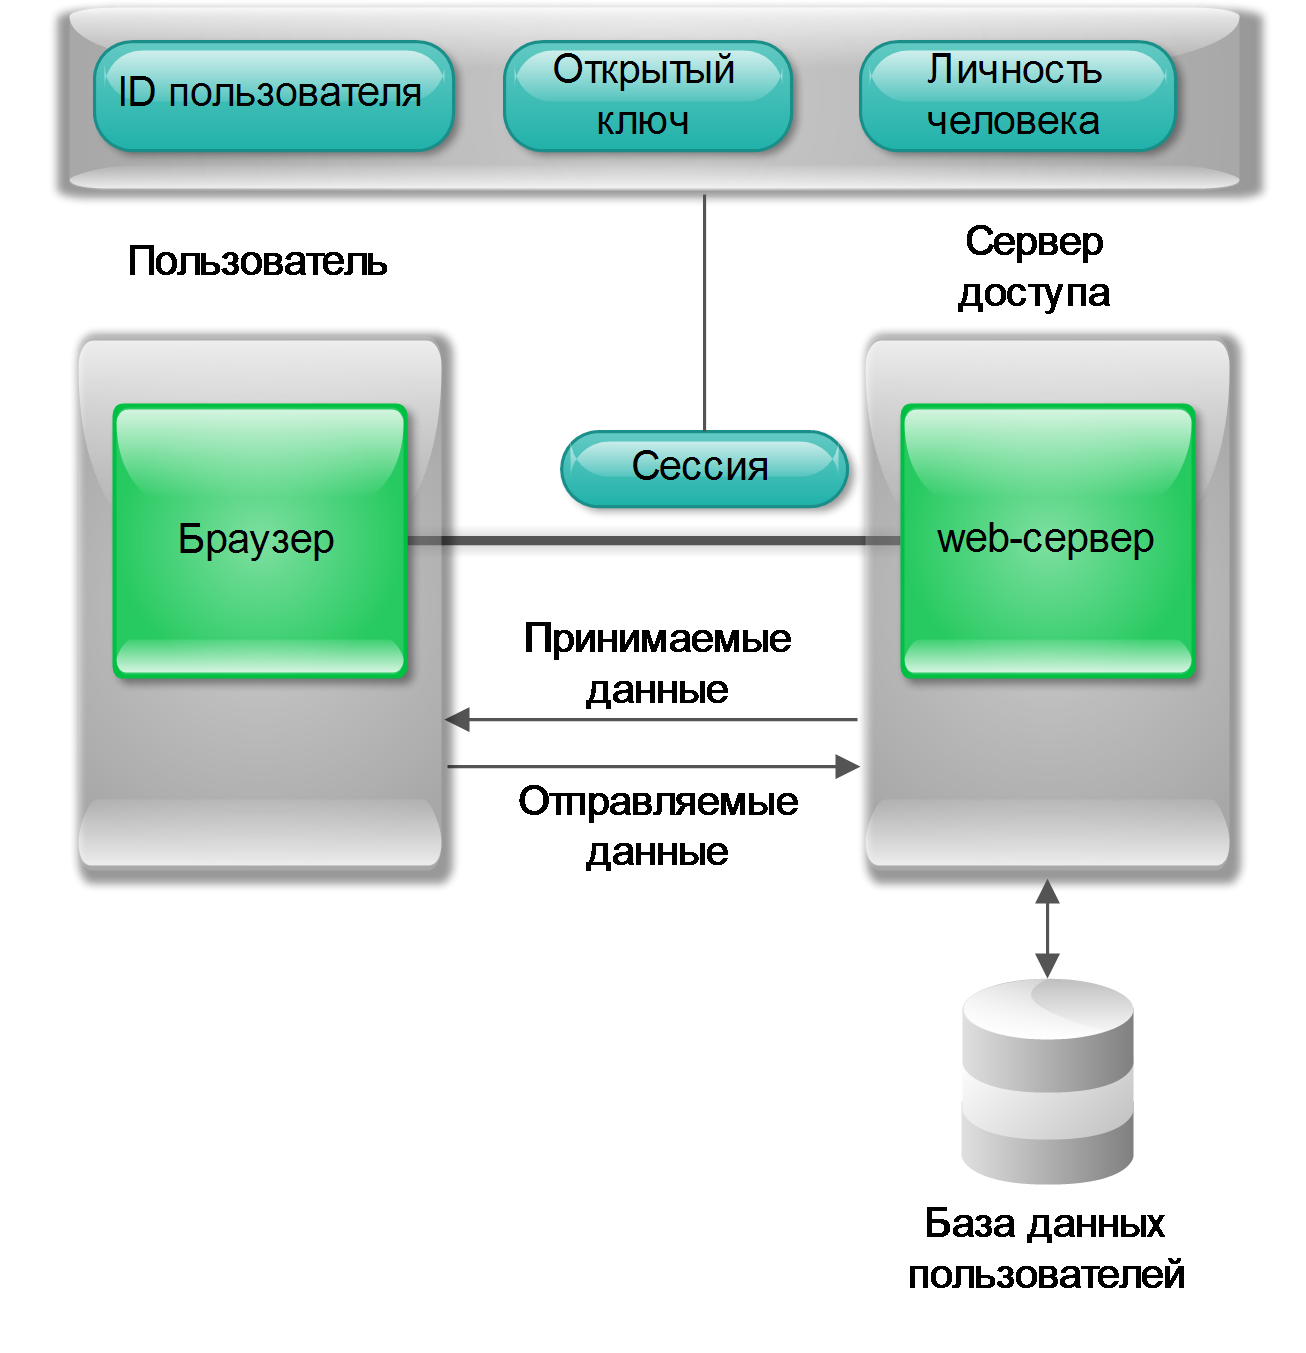
\includegraphics[width=1\linewidth]{3-1-3}}
\caption{Схема взаимодействия пользователя с сервером доступа}
\label{ris:3.1.3}
\end{figure} 
 
Пользователь через web-браузер соединяется с сервером доступа, и,
проходя аутентификацию, устанавливается сессия, в случае успешной проверки
подлинности пользователя. Возникает соответствие между идентификатором
пользователя в сети, личностью человека и его открытым ключом при
соответствующем обращении к базе данных.

В процессе аутентификации пользователю передаются данные в виде пакета
(получаемые данные) следующего содержания:
\begin{itemize}
  \item случайная последовательность (по другому ее называют <<соль>>);
  \item параметры алгоритма шифрования (они могут меняться с каждым разом);
  \item апплет – клиентская Web-программа, выступающая в роли согласующего звена
  между ПК и цифровым носителем закрытого ключа.
\end{itemize}

После проведения процедуры вычисления сигнатуры (шифра) на сервер отправляются
ответные данные включающие:
\begin{itemize}
  \item идентификатор пользователя в системе;
  \item сигнатура.
\end{itemize}

Полученная на сервере сигнатура закрепляется за конкретным пользователем,
определенным по его идентификатору, в рамках даннного сеанса. По данному
пользователю выбирается информация, необходимая для алгоритма проверки
подлинности сигнатуры (эта информация должна целиком существовать на сервере на
текущий момент), и осуществляется процедура верификации, в результате которой на
выходе получается положительный ответ, фиксируемый в базе данных в виде
создания сессии для пользователя, а так же в браузере клиента в виде
специального идентификатора сессии, задействовав технологию <<cookie>>.
В случае отрицательного ответа, от пользователя требуется проведение процедуры повторно, так как, вероятнее всего,
произошла подмена.

\begin{figure}[h!]
\center{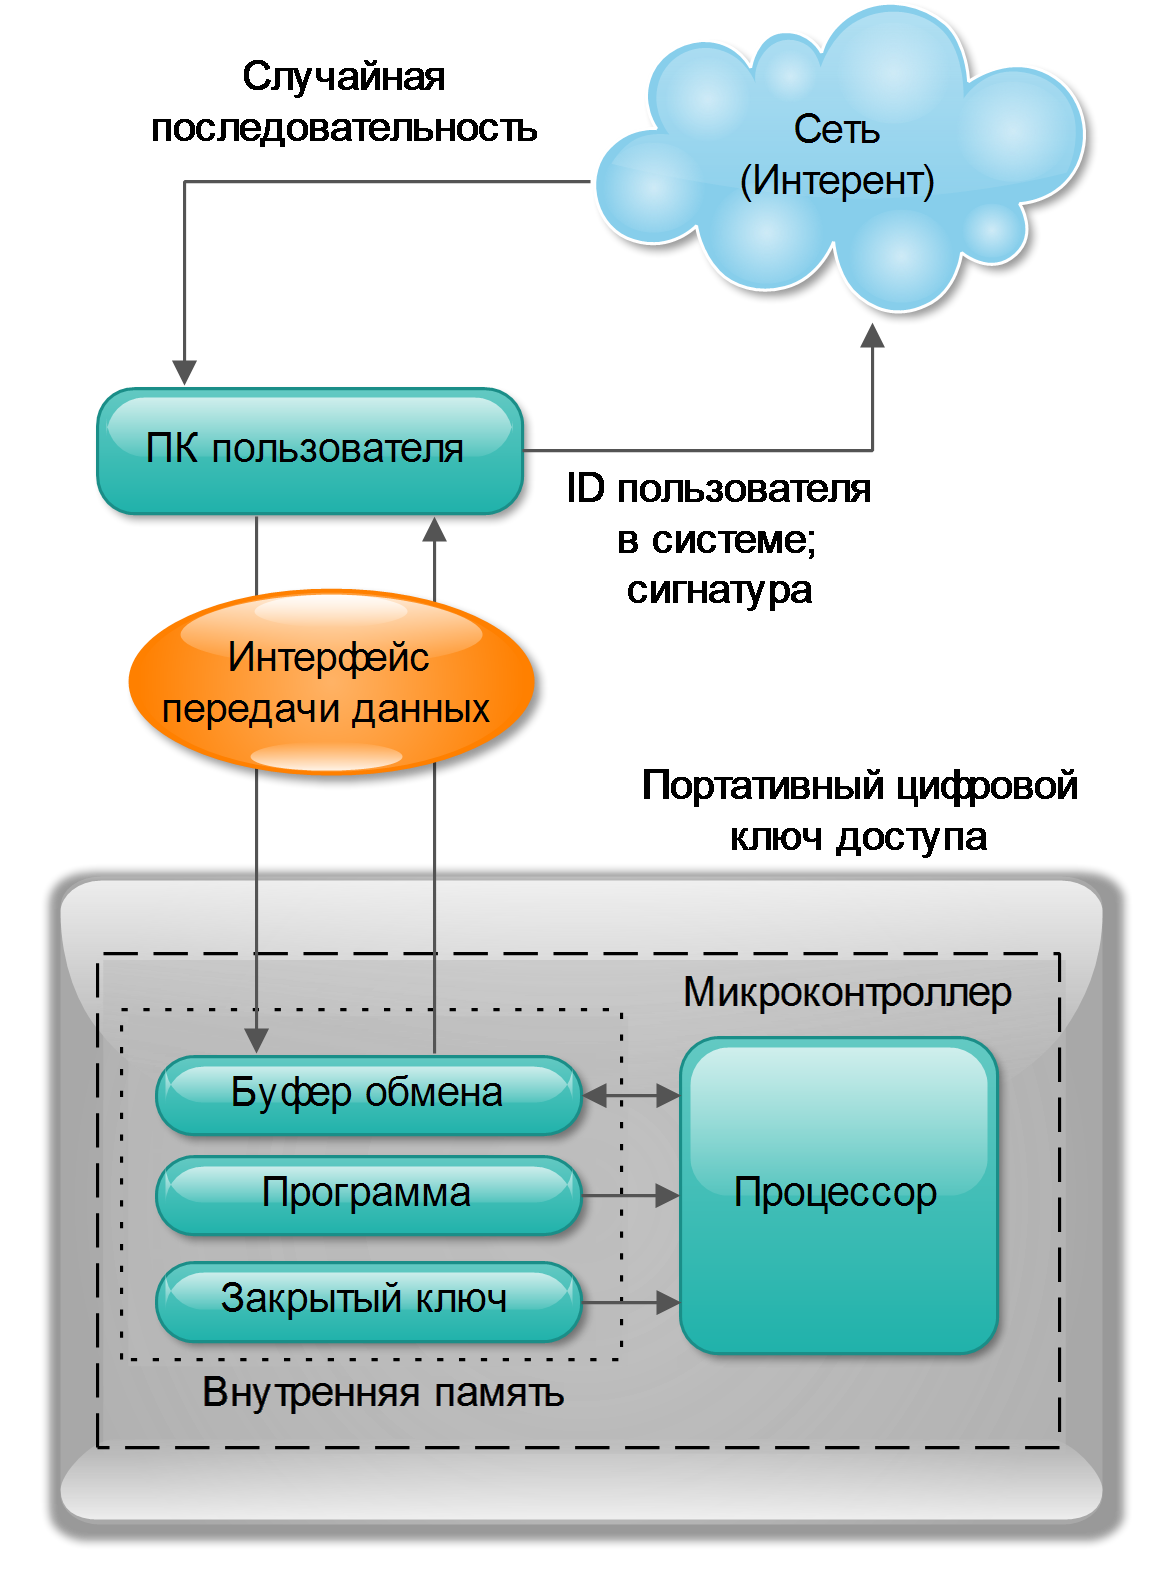
\includegraphics[width=0.6\linewidth]{3-1-4}}
\caption{Схема информационного обмена клиенской подсистемы в процессе
аутентификации}
\label{ris:3.1.4}
\end{figure} 

Схему, изображенную на рисунке~\ref{ris:3.1.3} можно детализировать с точки
зрения процессов, происходящих на стороне пользователя. Особую роль здесь играет
<<Портативный Цифровой Ключ Доступа>> (далее ПЦКД). Схема информационного обмена
клиенской подсистемы представлена на рисунке~\ref{ris:3.1.4}.

После получения пакета данных от сервера клиентская программа выполняет следующий ряд действий:
\begin{itemize}
  \item программа апплет устанавливает виртуальное соединение с носителем закрытого
ключа и получает ответ от согласующей программы, установленной на данном
носителе, об успешном подключении;
\item апплет запрашивает у пользователя короткий
код подтверждения, (PIN-код) тем самым дополнительно идентифицируя пользователя
как владельца данного носителя закрытого ключа. Данный код передаётся в
ПЦКД, который должен ответить положительным результатом. Система должны быть
оснащена защитой от взлома кода подбором;
\item апплет передает в ПЦКД случайную последовательность, полученную от
сервера доступа;
\item ПЦКД, получив на вход сообщение, вычисляет сигнатуру в соответствии с
алгоритмом, подгружая из памяти параметры алгоритма, идентификатор пользователя
в системе и закрытый ключ.
По окончании вычислений возвращает ответ на ПК;
\item апплет в свою очередь возвращает на сервер по открытому каналу полученные
данные, а так же идентификатор пользователя в системе.
\item финальным этапом является процедур верификации сигнатуры и установления
сессии.
\end{itemize}

Следует отметить что представленную технологию можно использовать как для
аутентификации пользователей, так и для проверки подлинности электронных
документов, не изменяя схему выполнения процесса, за исключением одного условия:
в качестве сообщения для выполнения алгоритмов будет выступать тело документа.
